3D компьютерная графика -- способ представления геометрической информации в трехмерном пространстве (зачастую представленной
в Декартовой системе координат), сохраненной на компьютере с целью произведения вычислений и создания двухмерных изображений.
Результирующие изображения могут быть в сохранены для просмотра в будущем, либо отображаться в реальном времени. \ref{figure:domain:utah}

\begin{figure}[ht]
\centering
  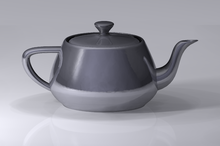
\includegraphics[scale=1.9]{utah_teapot.png}
  \caption{Изображение трехмерной модели Чайника Ньювелла}
  \label{figure:domain:utah}
\end{figure}


Процесс отображения 3D графики основан на многих алгоритмах работы с двухмерными векторными изображениями в стадии обработки
каркасов моделей (также называемых wireframe-моделями) и алгоритмах работы с растровой графикой при получении финального изображения.
Зачастую, из-за смешанного подхода к работе с трехмерной графикой, сложно выделить набор явных различий между 3D и 2D, так как многие
среды, предназначенные для работы с двухмерной графикой используют техники обработки трехмерных изображений (например, для достижения
реалистичной модели освещения), а системы работы с трехмерной графикой подразумевают использования техник обработки двухмерных изображений
(например, постобработка).

Понятие объектов трехмерной графики часто отождествляют с понятием 3D моделей, однако эти понятия не совсем тождественны,
так как модель по своей сути является лишь математическим представлением трехмерного объекта. Она не является производной
компьютерной графики до тех пор, пока не будет отображена на двухмерном изображении. Модель может быть отображена на изображении
в результате процесса, называемого <<3D-рендеринг>>, а также использована во всевозмжных не графических симуляциях либо вычислениях.
Еще одним применением трехмерных моделей, набирающим популярность в последние годы, можно называть 3D-печать. В случае трехмерной
печати, модель отображается из математического представления в реальный физический объект, однако, с некоторыми ограничениями, в
основном связаннными с предельной точностью печати.
